%
%-----------------------------------
\section{Line-broadening mechanisms}
\label{sec:line-broadening-mechanisms}
%-----------------------------------
%

In section \ref{sec:spectral-broadening}, we introduce the \textit{line shape function} $ g(\omega) $, which gives the probability of either absorbing or emitting a photon with a frequency between $ \omega $ and $ \omega + d\omega $. This function is proportional to the \textit{absorption cross-section} $ \sigma(\omega) $ according equation (\ref{eq:absorption-cross-section-2}). Although the line shape function take spectral broadening into account, it is not directly proportional to both absorbing and fluorescence profiles, which are actually measured. Theses profiles are associated directly with the \textit{net absorption cross-section} $ \sigma_{abs} $ and the \textit{scattering cross-section} $ \sigma_{sc} $. From equations (\ref{eq:net-absorption-cross-section-3}) and (\ref{eq:scattering-cross-section}), we can see that the absorption profile is not a sharp line as discussed in section \ref{sec:spectral-broadening}. In the next sections, we shall discuss physical effects which can both broaden and shift the absorption/scattering cross-section profile. Overall, there are two types of line broadening mechanisms: 
\begin{itemize}
	\item \textbf{Homogeneous broadening:} all atoms in a medium are affected in the same way. In this case, we can add these line-broadening mechanisms in the optical Bloch equations so that it is valid for all atoms in the medium;

	\item \textbf{Inhomogeneous broadening:} each atom in a medium is individually affected. In this case, we can only described line-broadening mechanisms in the optical Bloch equations for individual atoms. Therefore, we can not generalize for all atoms in the medium.
\end{itemize}

%-----------------------------------
\subsection{Natural broadening}
\label{sec:natural-broadening}
%-----------------------------------

Let us assume an isolated atom initially in the excited state so that there is not an incident light beam ($ s_0 = 0 $). This atom will decay in an average time $ 1/\Gamma $. In other words, $ 1 / \Gamma $ is the average time for the system changes considerably. Therefore, due to the \textit{time-energy uncertainty principle}, there will be an energy uncertainty in the excited state given by
\begin{equation}
	\Delta E \geq \frac{\hbar}{2\Delta t} = \frac{\hbar\Gamma}{2}.
\end{equation}
\begin{figure}[!ht]
	\centering
	\vspace{0pt}
	\caption{Natural broadening}
	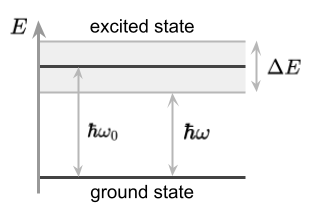
\includegraphics[width=0.4\textwidth]{USPSC-img/natural_broadening.png}
	\vspace{5pt}
	\legend{Energy uncertainty of a excited state whose lifetime is $ 1/\Gamma $. Due to the time-energy uncertainty principle, $ \Delta E \geq \hbar \Gamma / 2 $ and then a spontaneously emitted photon have a random energy $ \hbar \omega $ whose the average is $ \hbar \omega_0 $ and the uncertainty is greater than $ \hbar \Gamma / 2 $.\\ Source: Author}
	\vspace{-10pt}
	\label{fig:natural-broadening}
\end{figure}
Spontaneously emitted photons do not have a deterministic energy $ \hbar \omega_0 $ since the system does not have either, as illustrated in figure \ref{fig:natural-broadening}. This phenomena provokes a \textit{homogeneous} line-broadening known as \textbf{natural broadening} or \textbf{lifetime broadening}. The probability of spontaneously emitting a photon with frequency between $ \omega $ and $ \omega + d\omega $ is given by the line shape function $ g(\omega) $ and it is proportional to the absorption cross-section $ \sigma(\omega) $ according equations (\ref{eq:line-shape-function-2}) and (\ref{eq:absorption-cross-section-3}). From equation (\ref{eq:line-shape-function-2}), we have
\begin{equation}
	g(\Delta) = \frac{1}{\pi} \frac{\Gamma / 2}{\Delta^2 + (\Gamma / 2)^2}.
	\label{eq:line-shape-function-natural-broadening}
\end{equation}
The equation (\ref{eq:line-shape-function-natural-broadening}) is \textit{Lorentzian profile} whose FWHM, also known as \textit{linewidth}, is $ \Gamma $, which is in agreement to equation (\ref{eq:line-shape-simplest-case}) proposed in section \ref{sec:spectral-broadening}. Since $ \Gamma $ is associated with the natural broadening, it is also called \textbf{natural linewidth}. In the regime of weak excitation so that $ s_0 \ll 1 $, the absorption cross-section approximately equals the net absorption cross-section such that $ \sigma \simeq \sigma_{abs} $.
 
%-----------------------------------
\subsection{Power broadening}
\label{sec:power-broadening}
%-----------------------------------

In the presence of a light field so that $ s_0 > 0 $, the only spectral broadening is the natural broadening given by (\ref{eq:line-shape-function-natural-broadening}). However, the net absorption cross-section $ \sigma_{abs} $ does not equal the absorption cross-section $ \sigma $. According to equation (\ref{eq:net-absorption-cross-section-2}), there will be a decreasing by a factor of $ 1 + s(\omega) $, which causes a line-broadening illustrated in figure (\ref{fig:net-absorption-cross-section}). From equations (\ref{eq:net-absorption-cross-section-3}) and (\ref{eq:absorption-cross-section-3}), we have
\begin{gather}
	\sigma(\Delta) = \frac{\pi \Gamma \sigma_0}{2} g(\Delta)\ \ \textrm{and}\ \ \sigma_{abs}(\Delta) = \frac{\pi \Gamma \sigma_0}{2(1 + s_0)} L(\Delta), 
	\\
	\textrm{where}\ \ L(\Delta) \equiv \frac{2}{\pi \Gamma'} \frac{1}{1 + (2\Delta / \Gamma')^2}\ \ \textrm{and}\ \ \Gamma' \equiv \Gamma \sqrt{1 + s_0}.
	\label{eq:absorption-line-shape}
\end{gather}
The function $ L $ is known as \textbf{absorption line-shape} and it is a \textit{Lorentzian profile} whose \textit{FWHM} is $ \Gamma' $. The quantity $ \Gamma' $ is known as \textbf{power-broadened linewidth}. In the regime of weak excitation so that $ s_0 \ll 1 $, the absorption line-shape becomes the line shape function, $ L(\Delta) \rightarrow g(\Delta) $, and the power-broadened linewidth becomes the natural linewidth, $ \Gamma' \rightarrow \Gamma $.

\begin{figure}[!ht]
	\centering
	\caption{Net absorption cross-section}
	\vspace{-5pt}
	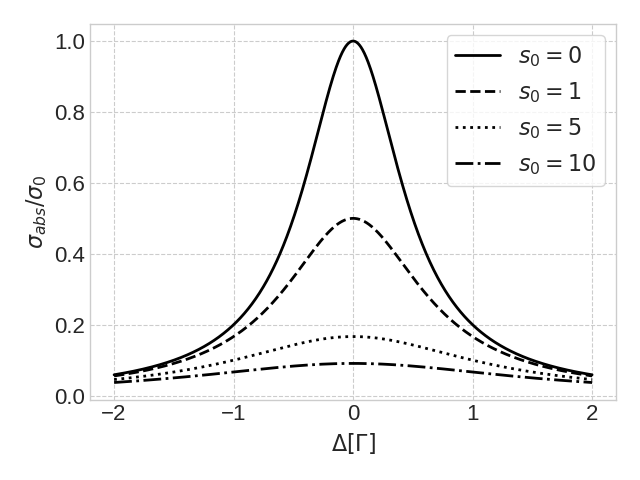
\includegraphics[width=0.5\textwidth]{USPSC-img/net_absorption_cross_section.png}
	\vspace{-5pt}
	\legend{Net absorption cross section as function of detuning for some values of resonant saturation parameter.\\ Source: Author}
	\label{fig:net-absorption-cross-section}
\end{figure}

%-----------------------------------
\subsection{Doppler broadening}
\label{sec:Doppler-broadening}
%-----------------------------------

The angular frequency $ \omega' $ of an incident light beam depends on the frame in which it is being observed. This effect is known as \textbf{Doppler effect}. We have been studying the atom-light interaction assuming that the light frequency is the same in both laboratory and atom frames. However, the Doppler effect causes an \textit{inhomogeneous resonance shift} since each atom will perceive an angular frequency given by
\begin{equation}
	\omega' = \omega - \mathbf{k} \cdot \mathbf{v},
	\label{eq:Doppler-effect}
\end{equation}
where $ \omega $ and $ \mathbf{k} $ are, respectively, the angular frequency and the wave vector of the light beam in the laboratory frame, and $ \mathbf{v} $ is the velocity of the atom also in the laboratory frame. Subtracting the resonant angular frequency $ \omega_0 $ in both sides of equation (\ref{eq:Doppler-effect}), we obtain
\begin{equation}
	\Delta_{eff} = \Delta - \mathbf{k} \cdot \mathbf{v},
	\label{eq:Doppler-shift}
\end{equation}
where $ \Delta_{eff} = \omega' - \omega_0 $ is the \textit{effective detuning}. We must called $ -\mathbf{k} \cdot \mathbf{v} $ as \textbf{Doppler shift}. Let us consider a gas following the \textit{Maxwell-Boltzmann distribution} so that the probability $ P(v) dv $ of finding an atom with a velocity component between $ v $ and $ v + dv $ parallel to $ \mathbf{k} $ direction is given by
\begin{equation}
	P(v) dv = \frac{1}{\alpha\sqrt{2\pi}} \exp\left(-\frac{v^2}{2\alpha^2}\right) dv,\ \ \alpha \equiv \sqrt{\frac{k_B T}{m}},
	\label{eq:Maxwell-Boltzmann-distribution}
\end{equation}
where $ T $ is the temperature of the gas, $ k_B $ is the Boltzmann constant, and $ m $ is the atom mass. The equation (\ref{eq:Maxwell-Boltzmann-distribution}) is a \textbf{Gaussian distribution} centered at zero whose \textit{standard deviation} is $ \alpha $. Also, the FWHM is approximately $ 2.355 \alpha $. If we consider a resonant laser so that $ \Delta = 0 $ or $ \omega = \omega_0 $, we can associated an effective absorption line shape given by
\begin{equation}
	D(\omega') = \frac{1}{\beta \sqrt{2\pi}} \exp\left[-\frac{(\omega' - \omega_0)^2}{2\beta^2}\right],\ \ \beta \equiv \frac{\omega_0}{c} \alpha = \frac{\omega_0}{c} \sqrt{\frac{k_b T}{m}}.
\end{equation}